\documentclass{article}

\usepackage[utf8]{inputenc}

\usepackage{amsmath, bm}
\usepackage{graphicx}
\usepackage{amssymb}
\usepackage{float}
\usepackage{caption}
\usepackage{subcaption}
\usepackage{hyperref}
\usepackage{tikz}
\usepackage{layout}
\usepackage{booktabs}

\usepackage[margin=1in]{geometry}
\usepackage{listings}
\usepackage{xcolor}
\usepackage{color, colortbl}
\usepackage{textgreek}
\usepackage{mathrsfs}

\usetikzlibrary{calc}
\usetikzlibrary{angles,quotes} % for pic
\usetikzlibrary{patterns,snakes}
\usetikzlibrary{arrows}
\tikzset{>=latex} % for LaTeX arrow head

\setlength{\parskip}{\baselineskip}%
\setlength{\parindent}{0pt}%
\linespread{0.9}


\definecolor{codegreen}{rgb}{0,0.6,0}
\definecolor{codegray}{rgb}{0.5,0.5,0.5}
\definecolor{codepurple}{rgb}{0.58,0,0.82}
\definecolor{backcolour}{rgb}{0.95,0.95,0.92}

\lstdefinestyle{mystyle}{
    backgroundcolor=\color{backcolour},   
    commentstyle=\color{codegreen},
    keywordstyle=\color{magenta},
    numberstyle=\tiny\color{codegray},
    stringstyle=\color{codepurple},
    basicstyle=\ttfamily\footnotesize,
    breakatwhitespace=false,         
    breaklines=true,                 
    captionpos=b,                    
    keepspaces=true,                 
    numbers=left,                    
    numbersep=5pt,                  
    showspaces=false,                
    showstringspaces=false,
    showtabs=false,                  
    tabsize=2
}

\lstset{style=mystyle}



\begin{document}

\title{Model Boat Retrofit}
\author{Louis}
\date{September 2025}
\maketitle 

\iffalse
\begin{abstract}
    \centering

\end{abstract}
\fi

%-----------------------------------------------------------------------------------------
\section{Introduction}
%-----------------------------------------------------------------------------------------

% introduction to model boating in cornwall

% unique nice design two keels

A model boat was given to me by my uncle Robin whom he recieved from his uncle Bill.
The boat has a unique twin keel design with the hull being carved from a solid block of wood.

\section{Objective}

With this project being the largest and most complex geometry the objectives were made to test and further my skills in engineering.
My background in aerospace engineering 

\begin{itemize}
    \item Produce an accurate 3D model of the curved hull shape.
    \item Perform quasi-static bouyancy analysis to predict float plane for optimal propeller placement.
    \item Retrofit the boat with a new electric propulsion system.
    \item Write firmware to control the boat remotely using drone radio control equipment.
\end{itemize}

\section{CAD Modelling}



\begin{figure}[H]
    \centering
    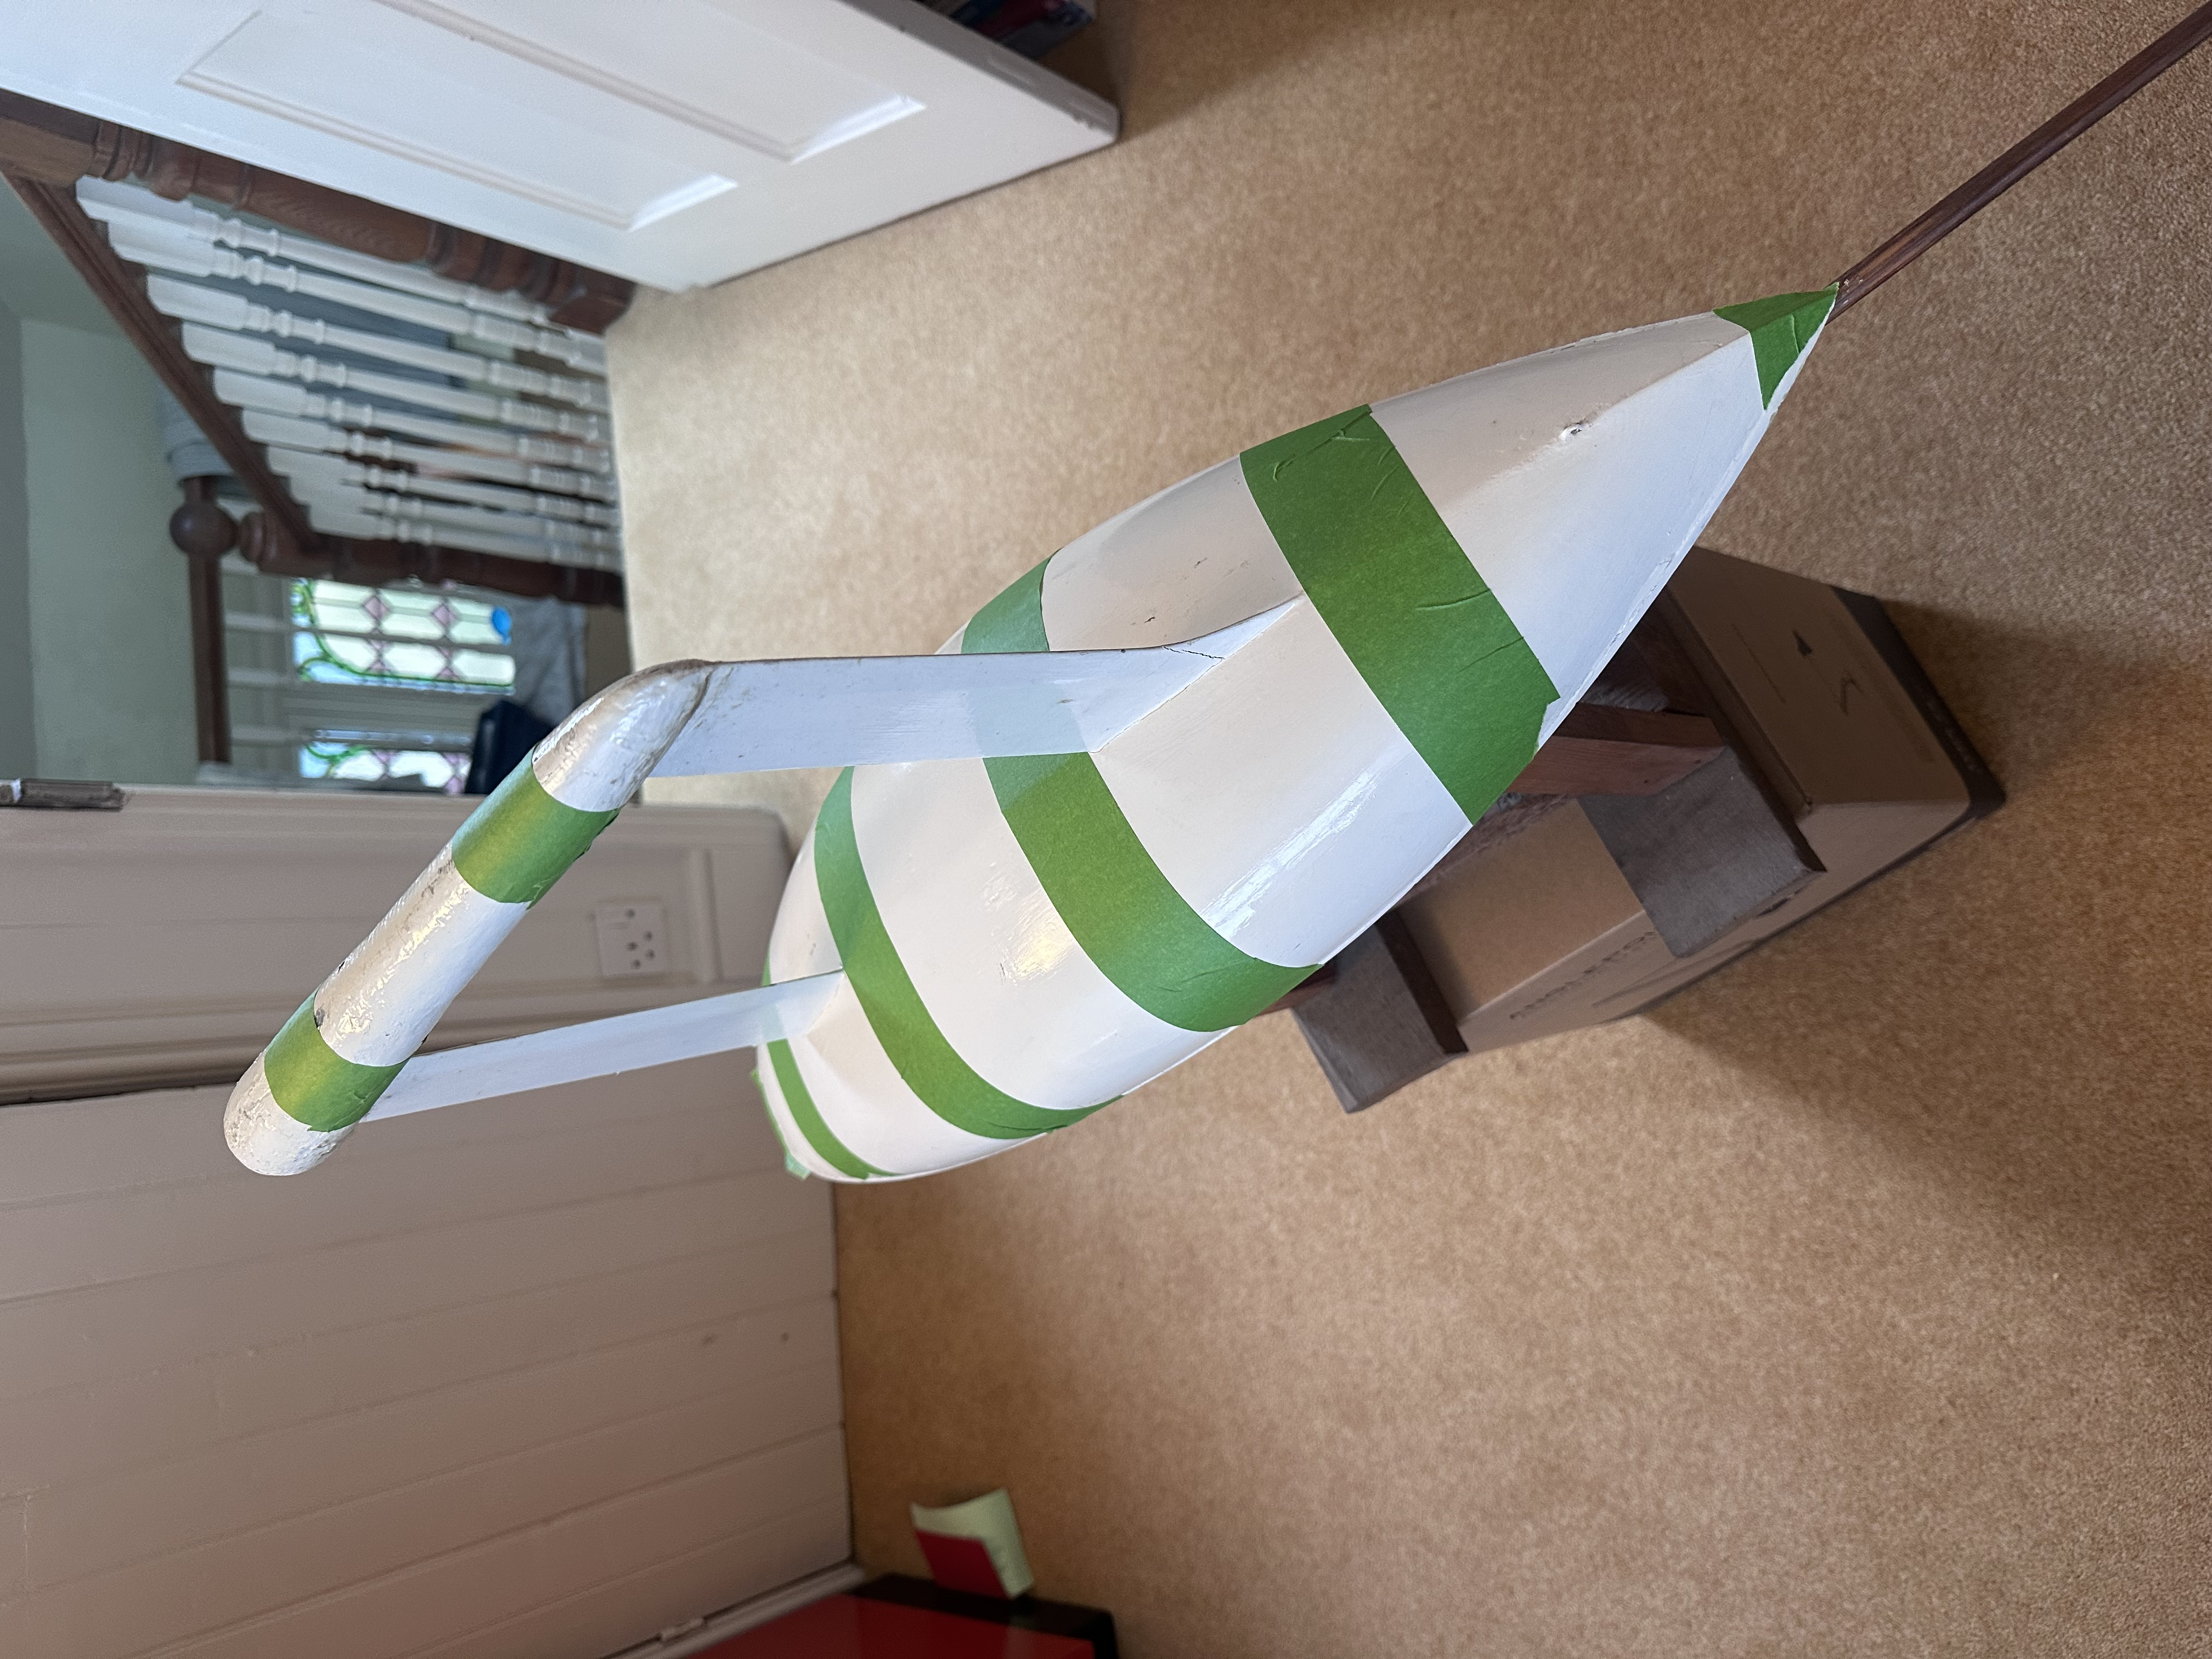
\includegraphics[width=0.8\textwidth]{figures/IMG_3011.jpg}
    \caption{Tape on boat hull to prevent lidar reflections.}
    \label{fig:lidar_tape}
\end{figure}

\begin{figure}[H]
    \centering
    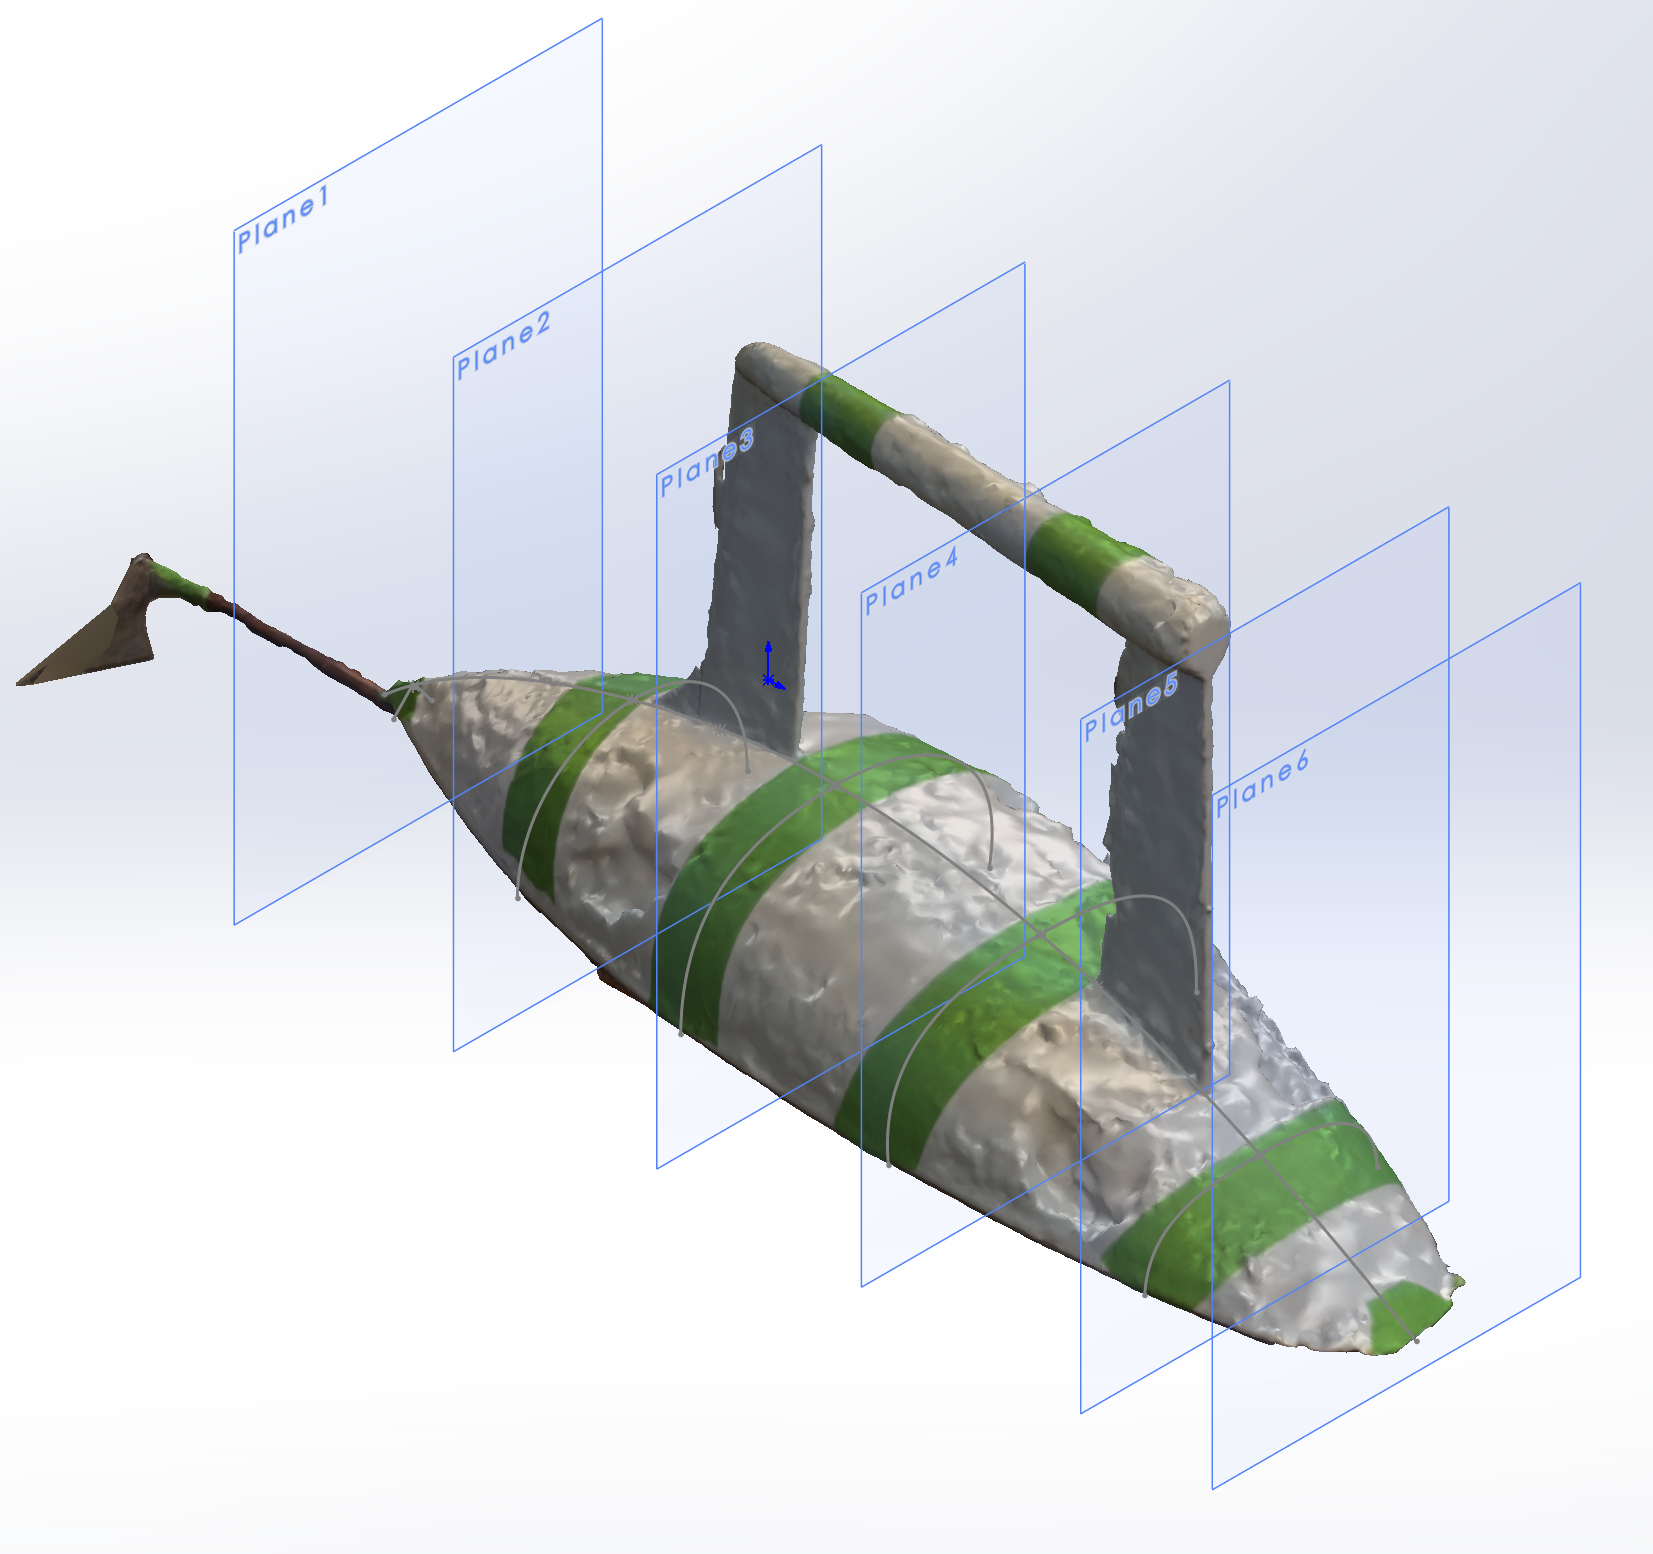
\includegraphics[width=0.8\textwidth]{figures/2m8uCHP5jN.png}
    \caption{3D scan of the boat hull in the CAD package SOLIDWORKS.}
    \label{fig:3d_scan}
\end{figure}

Splines were drawn on the lines of tape which were the smoothest, most geometrically accurate parts of the scanned hull.
Large holes can be seen on the reflective white areas of the hull which was where lidar rays reflected, tricking the scanner into thinking the hull was further away than it actually was.
The splines were then lofted to create a smooth hull surface.
More complex features 

\section{Bouyancy Analysis}

It will be relevant to discuss some theory of bouyancy before discussing the analysis.

Archimedes' principle states that a body submerged in a fluid experiences an upward force equal to the weight of the fluid it displaces.
For the body to be in equilibrium, the bouyancy force must equal the weight of the body.
This simply means we must displace the volume of water that has the same weight as the boat.
However, the average location of the boats weight, known as the center of gravity (CG),
may be different to the averaged location of displaced fluid, known as the center of bouyancy (CB).
This is because even for a boat with evenly distributed weight (uniform density), the submerged volume will be different to the total volume.

When these two points are not aligned, a moment will be created which will cause the boat to rotate until equilibrium is reached.
When CG is aligned vertically above CB, it is possible to be in an unstable equilibrium where a small perturbation will cause the boat to capsize.
A stable equilibrium is reached when CG is vertically below CB, where a small perturbation will create a restoring moment to return the boat to equilibrium.
When CG is further below CB, a larger restoring moment exists and boat can roll to a more extreme angle before becoming unstable and capsizing.
This is why boats have dense keels, to lower the CG and increase stability.

To determine the float plane of the boat, a quasi-static bouyancy analysis was performed in python.
The description 'quasi-static' is used because dynamic fluid forces are not considered as this would require far more complex CFD analysis.
It then follows that this is only valid when the boat rocks or settles at low speeds where dynamic fluid forces ($\rho V^2$) are negligible.

The 3D model was exported as an STL file and processed using the numpy-stl package.
A function is created to slice the mesh 

A simple gui was created to view how the boat settles over time from the quasi-static solver.
Upon loading an STL file and clicking the solve float plane button, an animation plays of the boat settling.
Euler angles (roll, pitch, yaw) are plotted over time to show how the boat stabilises.

\begin{figure}[H]
    \centering
    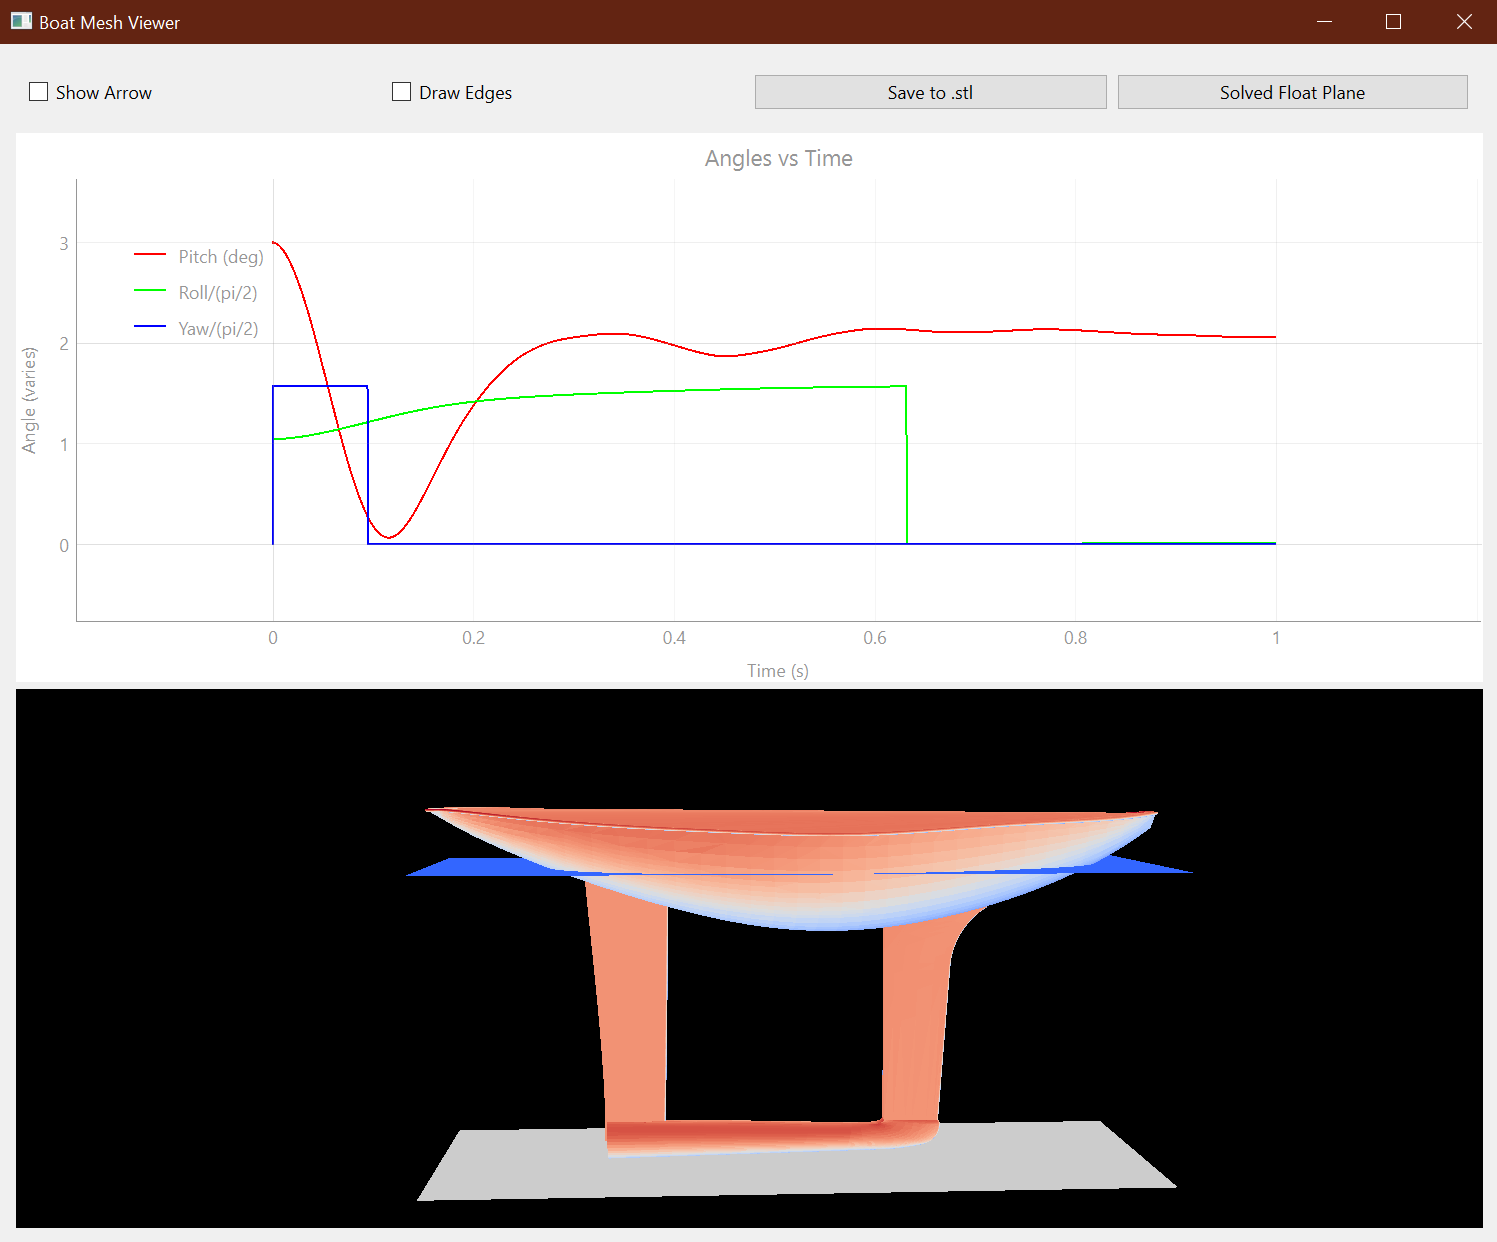
\includegraphics[width=0.8\textwidth]{figures/XqMwPnm3wm.png}
    \caption{Boat bouyancy analysis GUI.}
    \label{fig:boat_gui}
\end{figure}

Figure \ref{fig:boat_gui} shows the solver running with the boat model loaded.
It starts from a perturbed position (3 degrees pitch and 1 degree roll) and settles to a stable equilibrium.
Step changes are seen in the angle plots which may be due to the discontinuities in the volume calculation.
To understand this better, the calculation of submerged volume is explained.

The STL mesh is a series of triangular facets defined by three vertices and a normal vector.
To find the submerged volume, only the traingles with all three vertices below the waterline are considered.
A fourth vertex is taken as the point that defines the water plane and the submerged volume is the sum of tetrahedrons formed by each triangle and this fourth vertex.
The tetrahedron's volume is calculated using the determinant method.
\begin{equation}
    V = \frac{1}{6} \begin{vmatrix}
        x_1 & y_1 & z_1 & 1 \\
        x_2 & y_2 & z_2 & 1 \\
        x_3 & y_3 & z_3 & 1 \\
        x_4 & y_4 & z_4 & 1
    \end{vmatrix}
\end{equation}
The discontinuities in the angle plots are likely due to triangles that are on the edge of being submerged or not.
When a small change in angle causes a triangle to become submerged, it will cause a step change in the volume,
which over many iterations hidden in the x axis scale, causes steep changes in the angle plots.

A smooth response in pitch can be seen which converges nicely to a stable equilibrium of $\sim2$ degrees pitch up.



\section{Retrofitting work}

Holes were cut to fit a shaft for the propeller and rudder.
A large hole was cut in the top of the hull to fit the electronics and battery.
A temporary cover was 3D printed to seal the hole after the electronics were installed.
In the future this will be sealed either with an improved raised cabin or lowered cockpit.

* picture of big hole cut

A jig was made to drill the hole for the propeller shaft at the correct angle.
This was done by cutting the boat hull geometry from a block with a hole at the correct angle.
The block would then sit up against the keel and allow a precise hole to be drilled.
The shaft is then epoxied in place with the internal axel sealed with thick silicone grease to prevent water ingress.

* insert picture of jig
* insert picture of axel in place

The rudder was less straightforward due to limited hull space at the stern of the boat.
It was then decided to mount the rudder axel vertically through the hull.
A connecting rod above the hull then connects to the further bow side mounted servo, where the hull is deep enough to accommodate it.


\subsection{Hull modifications}

\subsection{Electronics and firmware}

Initially I planned to use a drone motor and ESC to power the propeller.
However, this was not feasible as these are designed to have a constant airflow over them to cool both the ESC and motor itself.
This is not possible in the enclosed hull of the boat.
High performance motors exist which use water cooling jackets, however these are expensive and surpasses the requirements of the project.
Instead, a brushed DC motor was used, driven by a high current H bridge motor driver.
These are much simpler devices which can be easily cooled with a small heatsink.
A 3s LiPo battery is used to power the motor, providing a nominal 11.1V and up to 20A of current.
The motor driver also has current shunt resistors, allowing the current to be measured by the rp2040 microcontroller.
It was originally planned to use a cheap 16 bit arudino based board, however, the remote control reciever required 32 bits to interface with it.
The rp2040 was chosen as a cheap but powerful microcontroller with a dual core ARM Cortex M0+ processor running at 133MHz.
The reciever also required 5V which can also be used to power the pico and so a regulator was used to step down the 11.1V battery supply.


\section{Conclusion}


\section{Appendix}



\begin{thebibliography}{9}

  \bibitem{handout}
  J. V. Taylor
  \emph{4A2 COMPUTATIONAL FLUID DYNAMICS: WRITING AN EULER SOLVER}
  University of Cambridge,
  2024.

\end{thebibliography}

\end{document}